\chapter{Standards} \label{ch:standarts}

Parallel development in different countries has led to various standards in the V2X communication. This thesis only considers the European standard from the European Telecommunications Standards Institute (ETSI). 

\section{IEEE 802.11p}

802.11p is an amendment of the WLAN standard IEEE 802.11-2012 optimized for the use in vehicular environment. It enables the communication between high-speed vehicles and roadside infrastructure (section \ref{sec:V2X-Communication}). 802.11p is covering the PHY and the MAC Layer and operates in the 5\;GHz band (5.850-5.925\;GHz) with 10\;MHz wide channels. \cite{IEEE802.11p}

802.11p is designed to increase road safety to meet specific requirements such as high reliability and low latency. With the 802.11p standard, message prioritization has been added to the MAC layer. This allows emergency messages to be prioritized. In addition, 802.11p is particularly suitable for establishing and forwarding connections quickly. \cite{Mustafa}

In Europe the term ITS-G5 is used for the access layer of the V2X system. ITS-G5 is based on the 802.11p standard. The main difference is the frequency allocation. It also operates in the 5\;GHz band but is split in four sub-parts as shown in figure \ref{fig:alloc}. \cite{ETSI_EN_302_663}


\begin{figure}[htb]
	\centering
	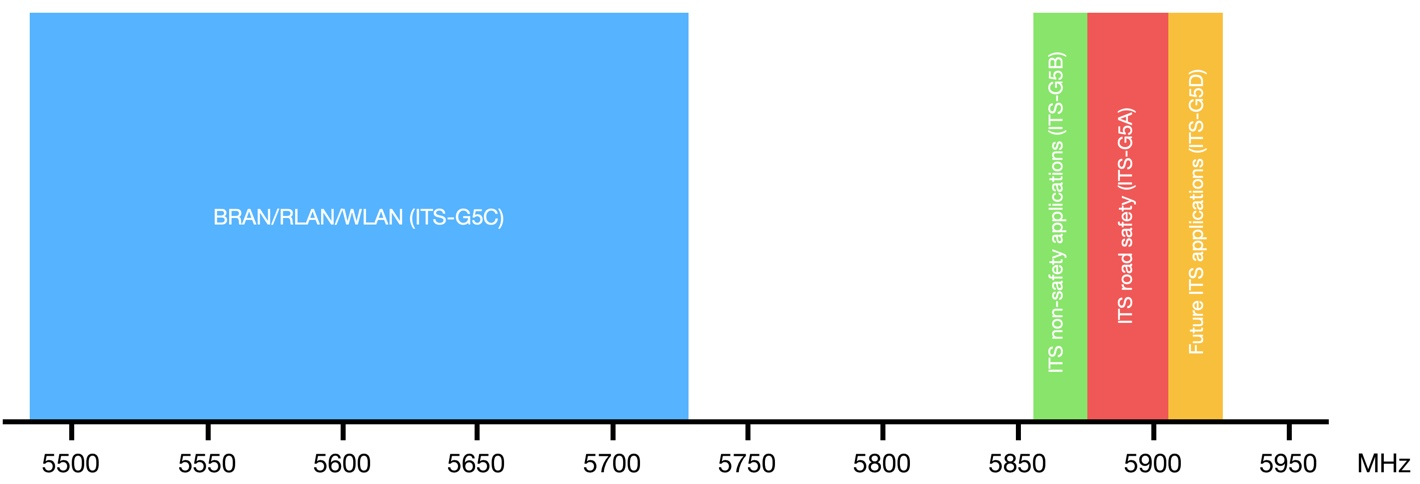
\includegraphics[width=0.8\textwidth]{images/f_allocation}
	\caption{Channel Allocation for the 5\;GHz Frequency Range}
	\label{fig:alloc}
\end{figure}

\section{C-V2X}

Unlike ITS-G5, C-V2X is based on LTE or in future 5G. The main advantage of C-V2X is, that it is based on newer mobile communication technology, has a higher data transfer rate and the ability to communicate directly between two stations or over a cellular network. \cite{CV2X}

\section{ETSI ITS}

ETSI ITS is the intelligent transport system in Europe. Figure \ref{fig:OSI_Model} shows the architecture of the ETSI ITS station compared to the OSI reference model. The three lower blocks contain the functionality of the OSI communication protocol stack. \cite{ETSI_EN_302_665}
\begin{itemize}
	\item "Access" representing ITSC's OSI layers 1 and 2
	\item "Networking \& Transport" representing ITSC's OSI layers 3 and 4
	\item "Facilities" representing ITSC's OSI layers 5, 6 and 7
\end{itemize}
 
\begin{figure}[htb]
	\centering
	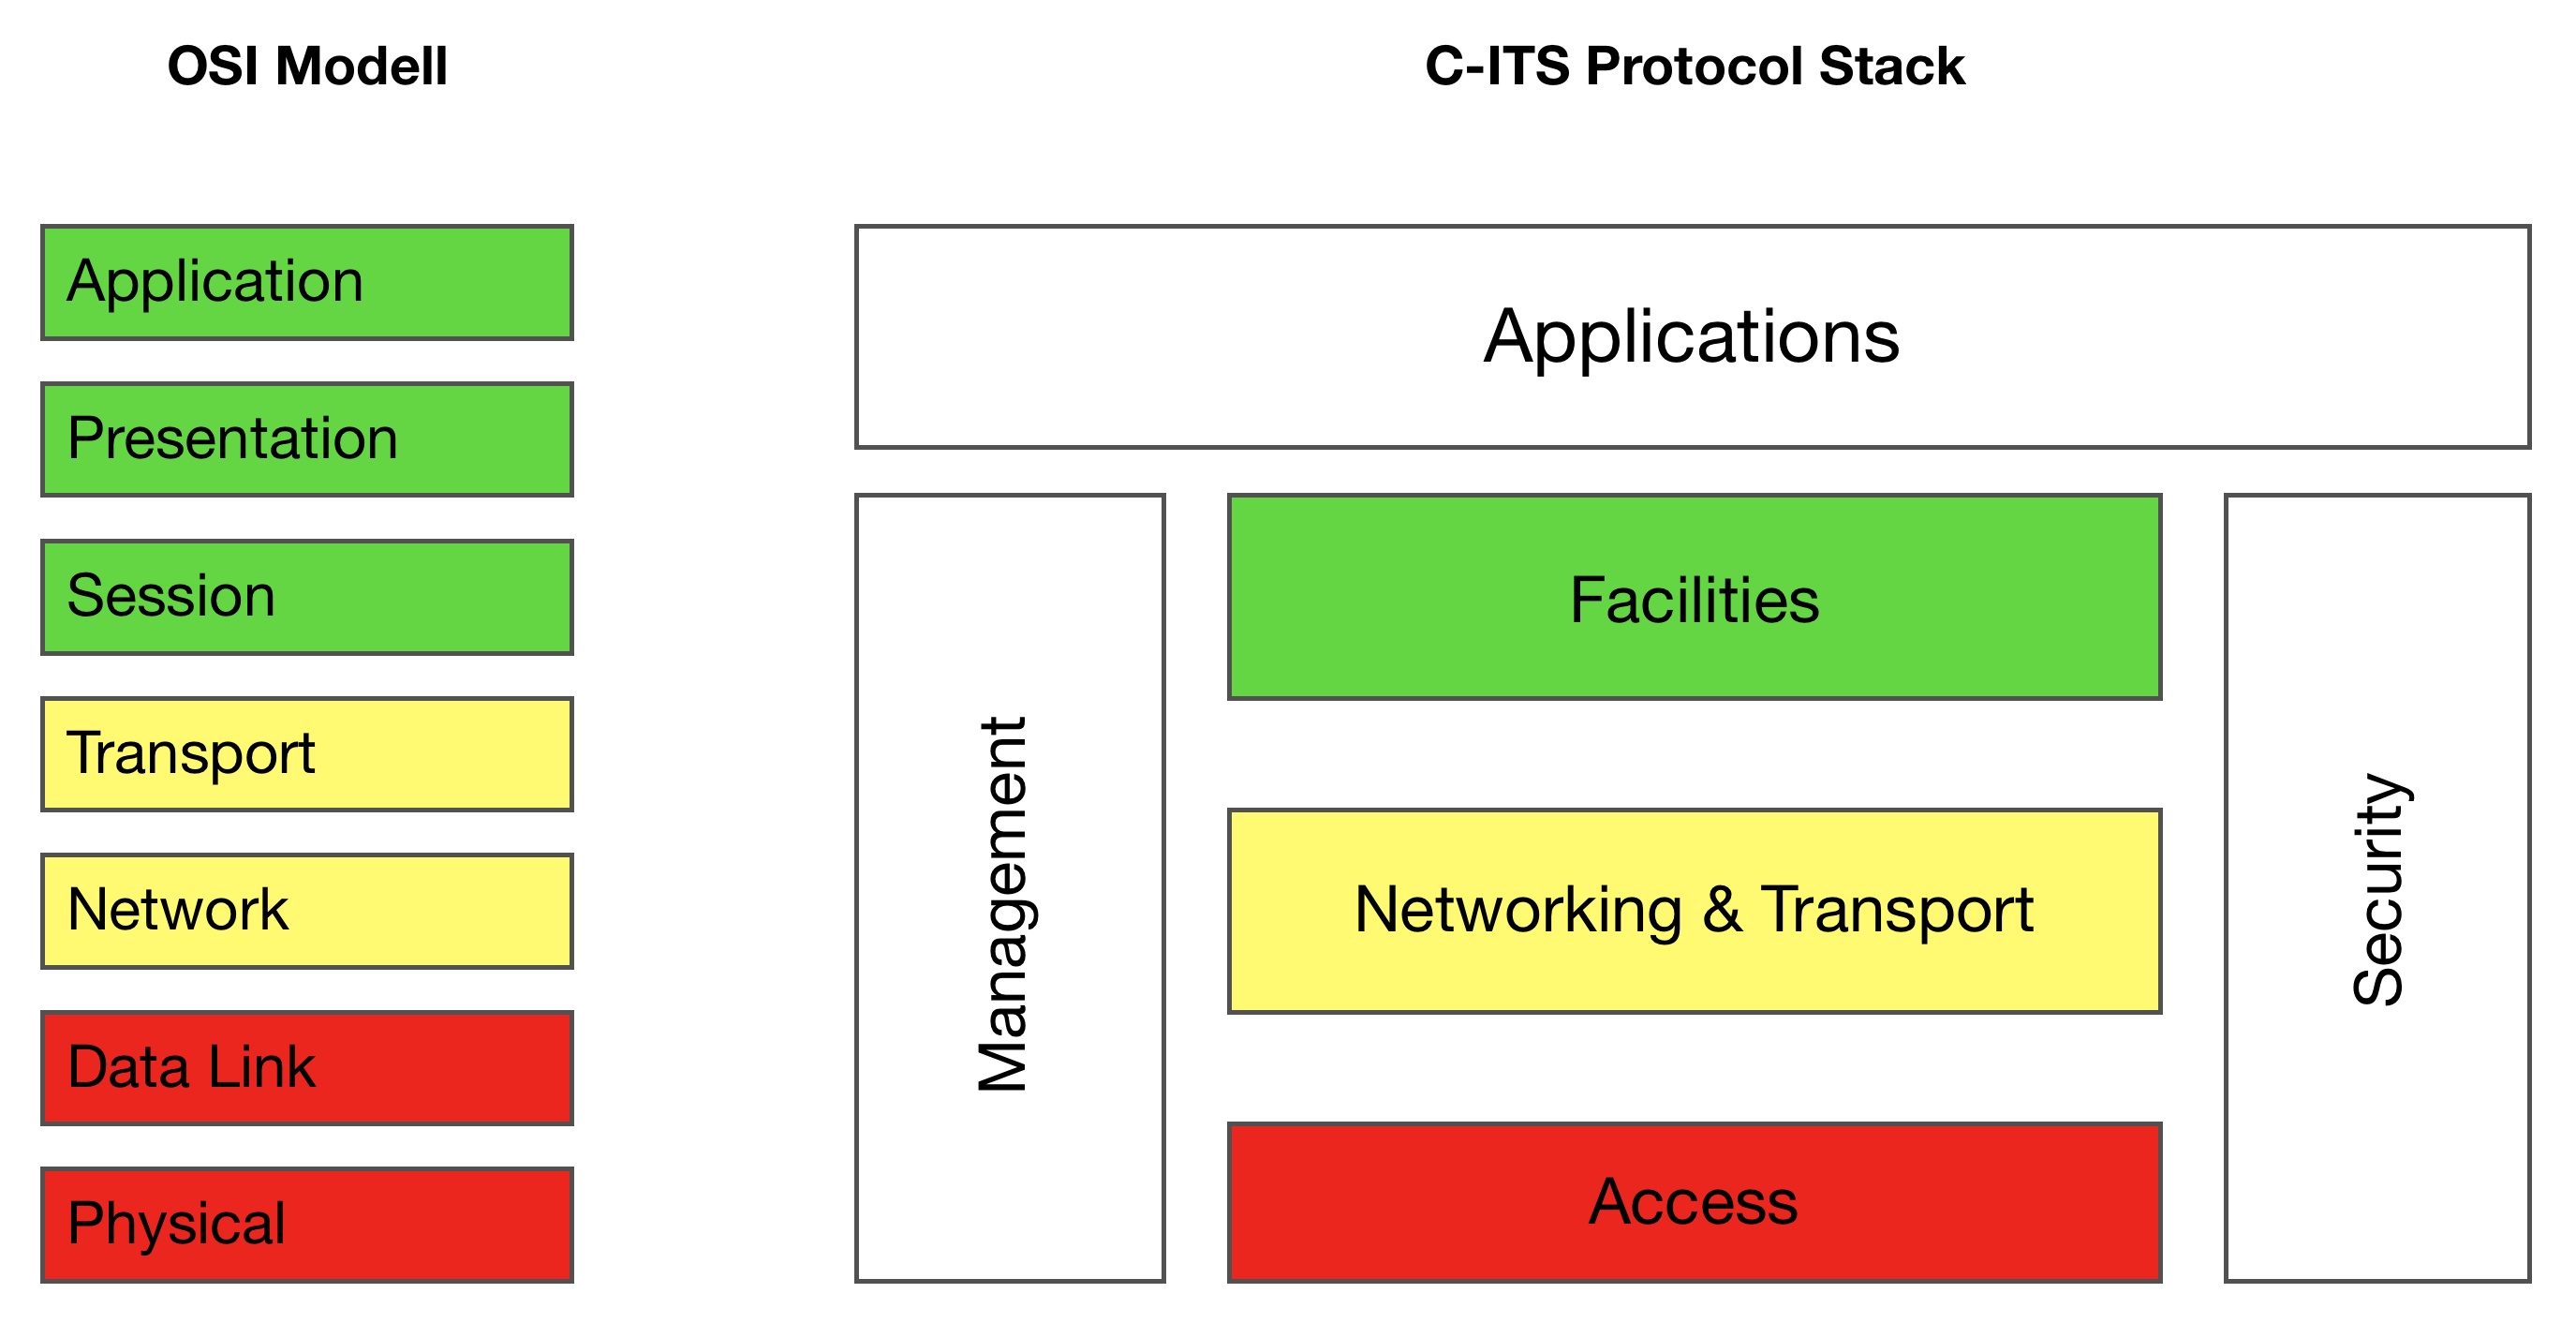
\includegraphics[width=0.6\textwidth]{images/OSI_Model}
	\caption{Architecture of ITS station}
	\label{fig:OSI_Model}
\end{figure}

\subsection{Access}
The PHY and the MAC are sublayers of the Access layer. The Access supports various wireless communication technologies, such as 802.11p and C-V2X.

\subsection{Networking and Transport}
In the Transport layer, protocols such as the Transmission Control Protocol (TCP), User Datagram Protocol (UDP) and Basic Transport Protocol (BTP) are implemented.

The Network layer provides network protocols as for example IPv4 and IPv6. This layer was extended by the GeoNetworking. \cite{ETSI_EN_302_665}

The GeoNetworking protocol and Basic Transport Protocol were specially designed for V2X applications. These two protocols allow broadcast messages to be restricted to a geographical area. Therefore, no direct addressing of a subscriber is necessary. All participants within the scope of the message receive it. This type of messages are called broadcast. \cite{Mustafa}

\newpage

\subsection{Facilities}

In this layer, messages such as the Cooperative Awareness Message (CAM) and the Decentralized Environmental Notification Messages (DENM) are defined. The information for these messages is generated and compiled at this level.

A CAM is sent periodically from each device in the ITS network. In a CAM, various information such as the time, position and movement status of vehicles are included.

A DENM is triggered by specific events. For example traffic jams, icy roads or accidents. It is used to notify other road users. \cite{ETSI_EN_302_665} \cite{Mustafa}

\subsection{Applications}

The Application layer is divided into three parts: "Road Safety", "Traffic Efficiency" and "Other Applications". \cite{ETSI_EN_302_665}

\subsection{Managment}

The Management layer controls various applications and the utilization of the channels. \cite{Mustafa}

\subsection{Security}

The Security layer provides security-relevant services. For example, the management of the firewall, the detection of unauthorized accesses, as well as their prevention. \cite{Mustafa}

\subsection{Basic Transport Protocol and GeoNetworking Protocol}\label{sec:BTP}

The Basic Transport Protocol (BTP) provides an end-to-end transport service in the ITS network. The main purpose of BTP is to multiplex and demultiplex the messages from different processes in the Facilities layer for the transmission over the GeoNetworking protocol.
The multiplexing and demultiplexing of different messages is based on ports. A port identifies the ITS station protocol entity at the source and the destination. The ports of BTP are similar to the ports in the internet protocol (IP). The IP provides the routing of the packets and UDP the multiplexing and demultiplexing of application processes messages. In this case, the GeoNetworking protocol transports the packets among the ITS stations (for example RSUs and OBUs) and the BTP protocol delivers the packet to the entities at the ITS Facilities layer. The BTP also adapts to the concept of "well-known ports" from the IP protocol, that assigns fixed ports to specific ITS Facilities layer protocols.  \cite{ETSI_TS_102_636-5-1}

The BTP data indication and request header is shown in appendix \ref{app:BTPHeaderIndicationRequest}.

\clearpage
\pagebreak